
\documentclass{article}

\usepackage{graphicx,hyperref}

\title{The \texttt{Typ2} mesh format}

\begin{document}

\maketitle

\section{Description of \texttt{typ2} format}

The \texttt{typ2} mesh format was designed for the FVCA5 benchmark \cite{bench}.
It describes a 2D mesh with generic polygonal cells in a txt file through the following elements:

\begin{verbatim}
Vertices
<nb Nv of vertices in the mesh>
<coordinates of vertex 1>
<coordinates of vertex 2>
.
.
.
<coordinates of vertex Nv>
cells
<nb Nc of cells in the mesh>
<nb of vertices of cell 1, followed by the ids of the vertices>
<nb of vertices of cell 2, followed by the ids of the vertices>
.
.
.
<nb of vertices of cell Nc, followed by the ids of the vertices>
\end{verbatim}

\textbf{Note}: for each cell, the vertices must be listed in counter-clockwise order.

\section{Examples}

Here are some examples of meshes in the directory.

\begin{center}
\begin{tabular}{cc}

\includegraphics[width=0.5\linewidth]{cart10x10.pdf} & 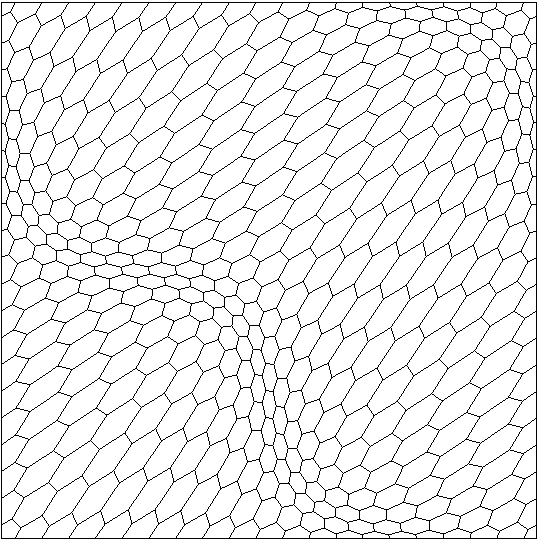
\includegraphics[width=0.5\linewidth]{hexa1_2.pdf}\\
{Member of the \texttt{cartXxX.typ2} family} & {Member of the \texttt{hexa1\_X.typ2} family}
\end{tabular}
\end{center}

\begin{center}
\begin{tabular}{cc}
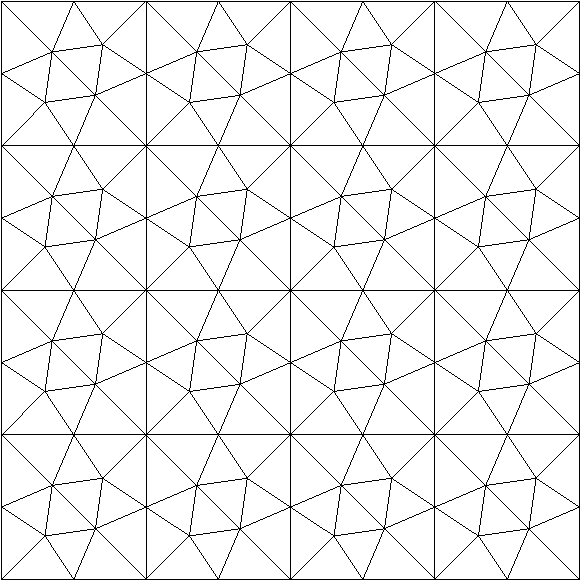
\includegraphics[width=0.5\linewidth]{mesh1_2.pdf} & 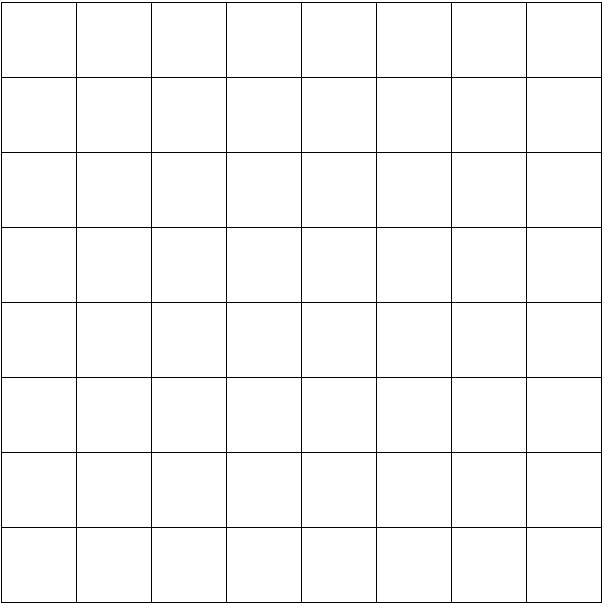
\includegraphics[width=0.5\linewidth]{mesh2_2.pdf} \\
{Member of the \texttt{mesh1\_X.typ2} family} & {Member of the \texttt{mesh2\_X.typ2} family}
\end{tabular}
\end{center}


\begin{center}
\begin{tabular}{cc}
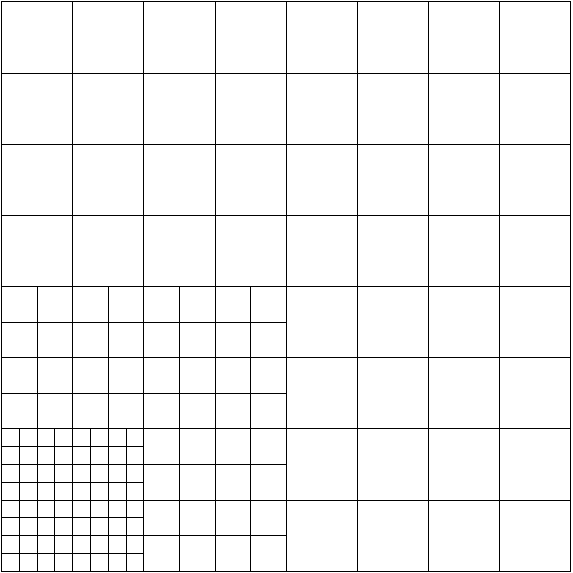
\includegraphics[width=0.5\linewidth]{mesh3_2.pdf} & 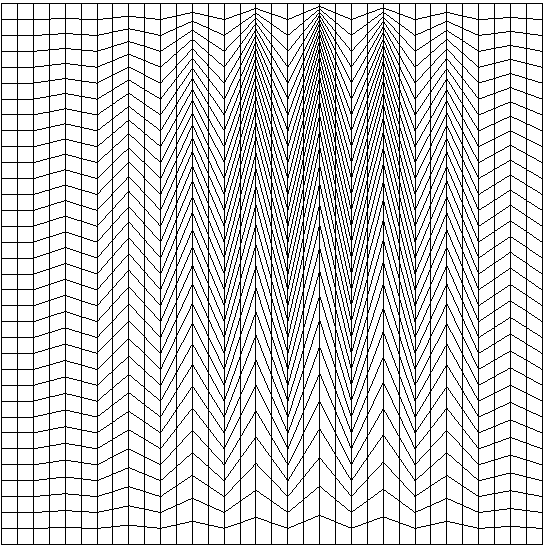
\includegraphics[width=0.5\linewidth]{mesh4_1_2.pdf}\\
{Member of the \texttt{mesh3\_X.typ2} family} & {Member of the \texttt{mesh4\_1\_X.typ2} family}
\end{tabular}
\end{center}


\begin{center}
\begin{tabular}{c}
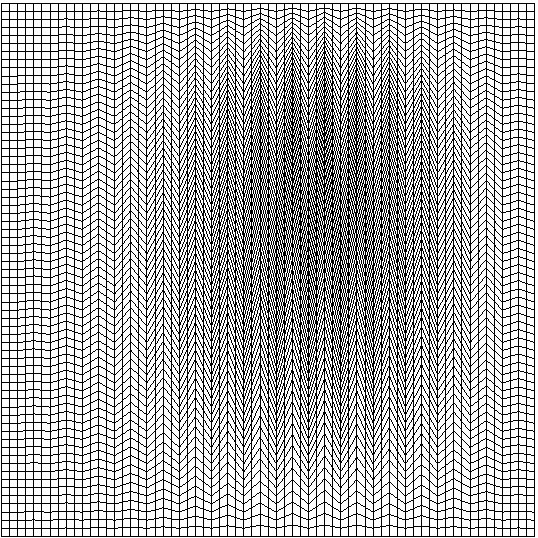
\includegraphics[width=0.5\linewidth]{mesh4_2_2.pdf}\\
{Member of the \texttt{mesh4\_2\_X.typ2} family}
\end{tabular}
\end{center}


%% Lshape

\begin{center}
\begin{tabular}{cc}
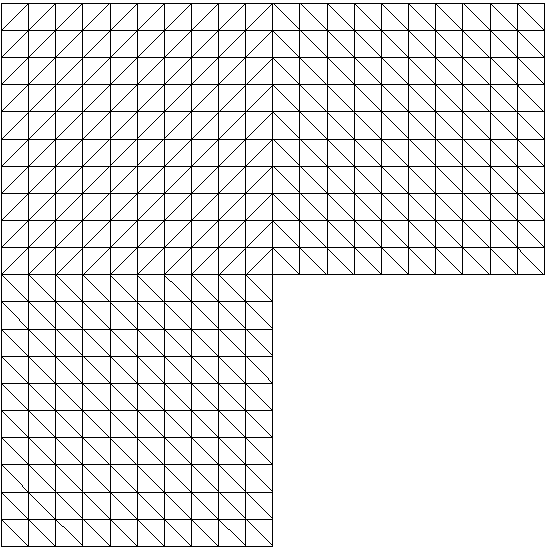
\includegraphics[width=0.5\linewidth]{Lshape_tri1_2.pdf} & 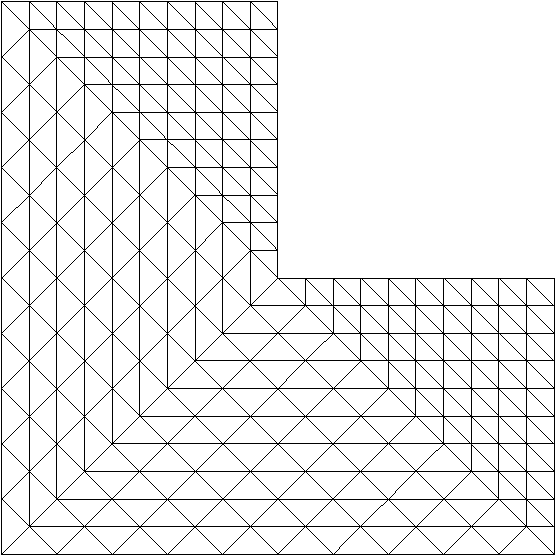
\includegraphics[width=0.5\linewidth]{Lshape_tri2.pdf}\\
{Member of the \texttt{Lshape\_tri1\_X.typ2} family} & {Member of the \texttt{Lshape\_triX.typ2} family}
\end{tabular}
\end{center}


\begin{center}
\begin{tabular}{c}
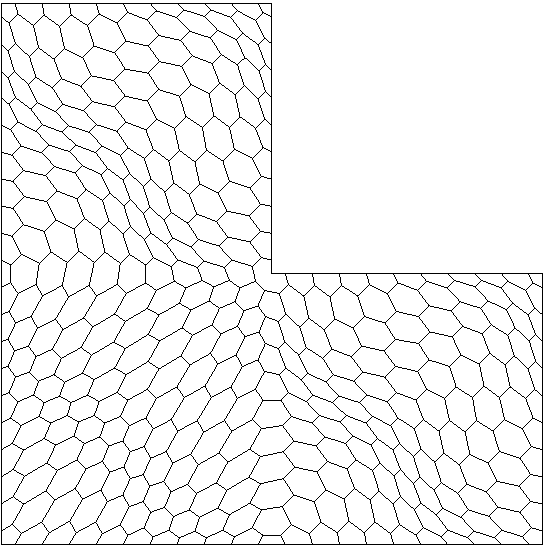
\includegraphics[width=0.5\linewidth]{Lshape_hexa2.pdf}\\
{Member of the \texttt{Lshape\_hexaX.typ2} family}
\end{tabular}
\end{center}

\begin{thebibliography}{99}

\bibitem{bench} R. Herbin, F. Hubert, \emph{Benchmark on discretization schemes for anisotropic diffusion problems
on general grids}, in Finite Volumes for Complex Applications V (ISTE, London, 2008), pp. 659--692.
URL: \href{http://www.i2m.univ-amu.fr/fvca5/benchmark/Meshes/index.html}{http://www.i2m.univ-amu.fr/fvca5/benchmark/Meshes/index.html}

\end{thebibliography}

\end{document}


